

\section{Introduction}
Financial markets are high-dimensional, non-stationary stochastic systems, where returns exhibit heavy tails \cite{fama1965behavior}, time-varying volatility \cite{engle1982autoregressive}, and cross-sectional dependence \cite{pesaran2021general}. Quantitative investment therefore relies on alpha mining to extract predictive signals from noisy observations. Recently, large language models (LLMs) \cite{lope2025chatgpt} and LLM-based agent frameworks \cite{zhang2024multi, xiao2025trad} have been introduced into the factor research workflow. By leveraging advanced reasoning and code generation capabilities, these systems can automate factor construction and iteratively refine candidates through backtesting feedback.

\begin{figure}[htbp]
    \centering
    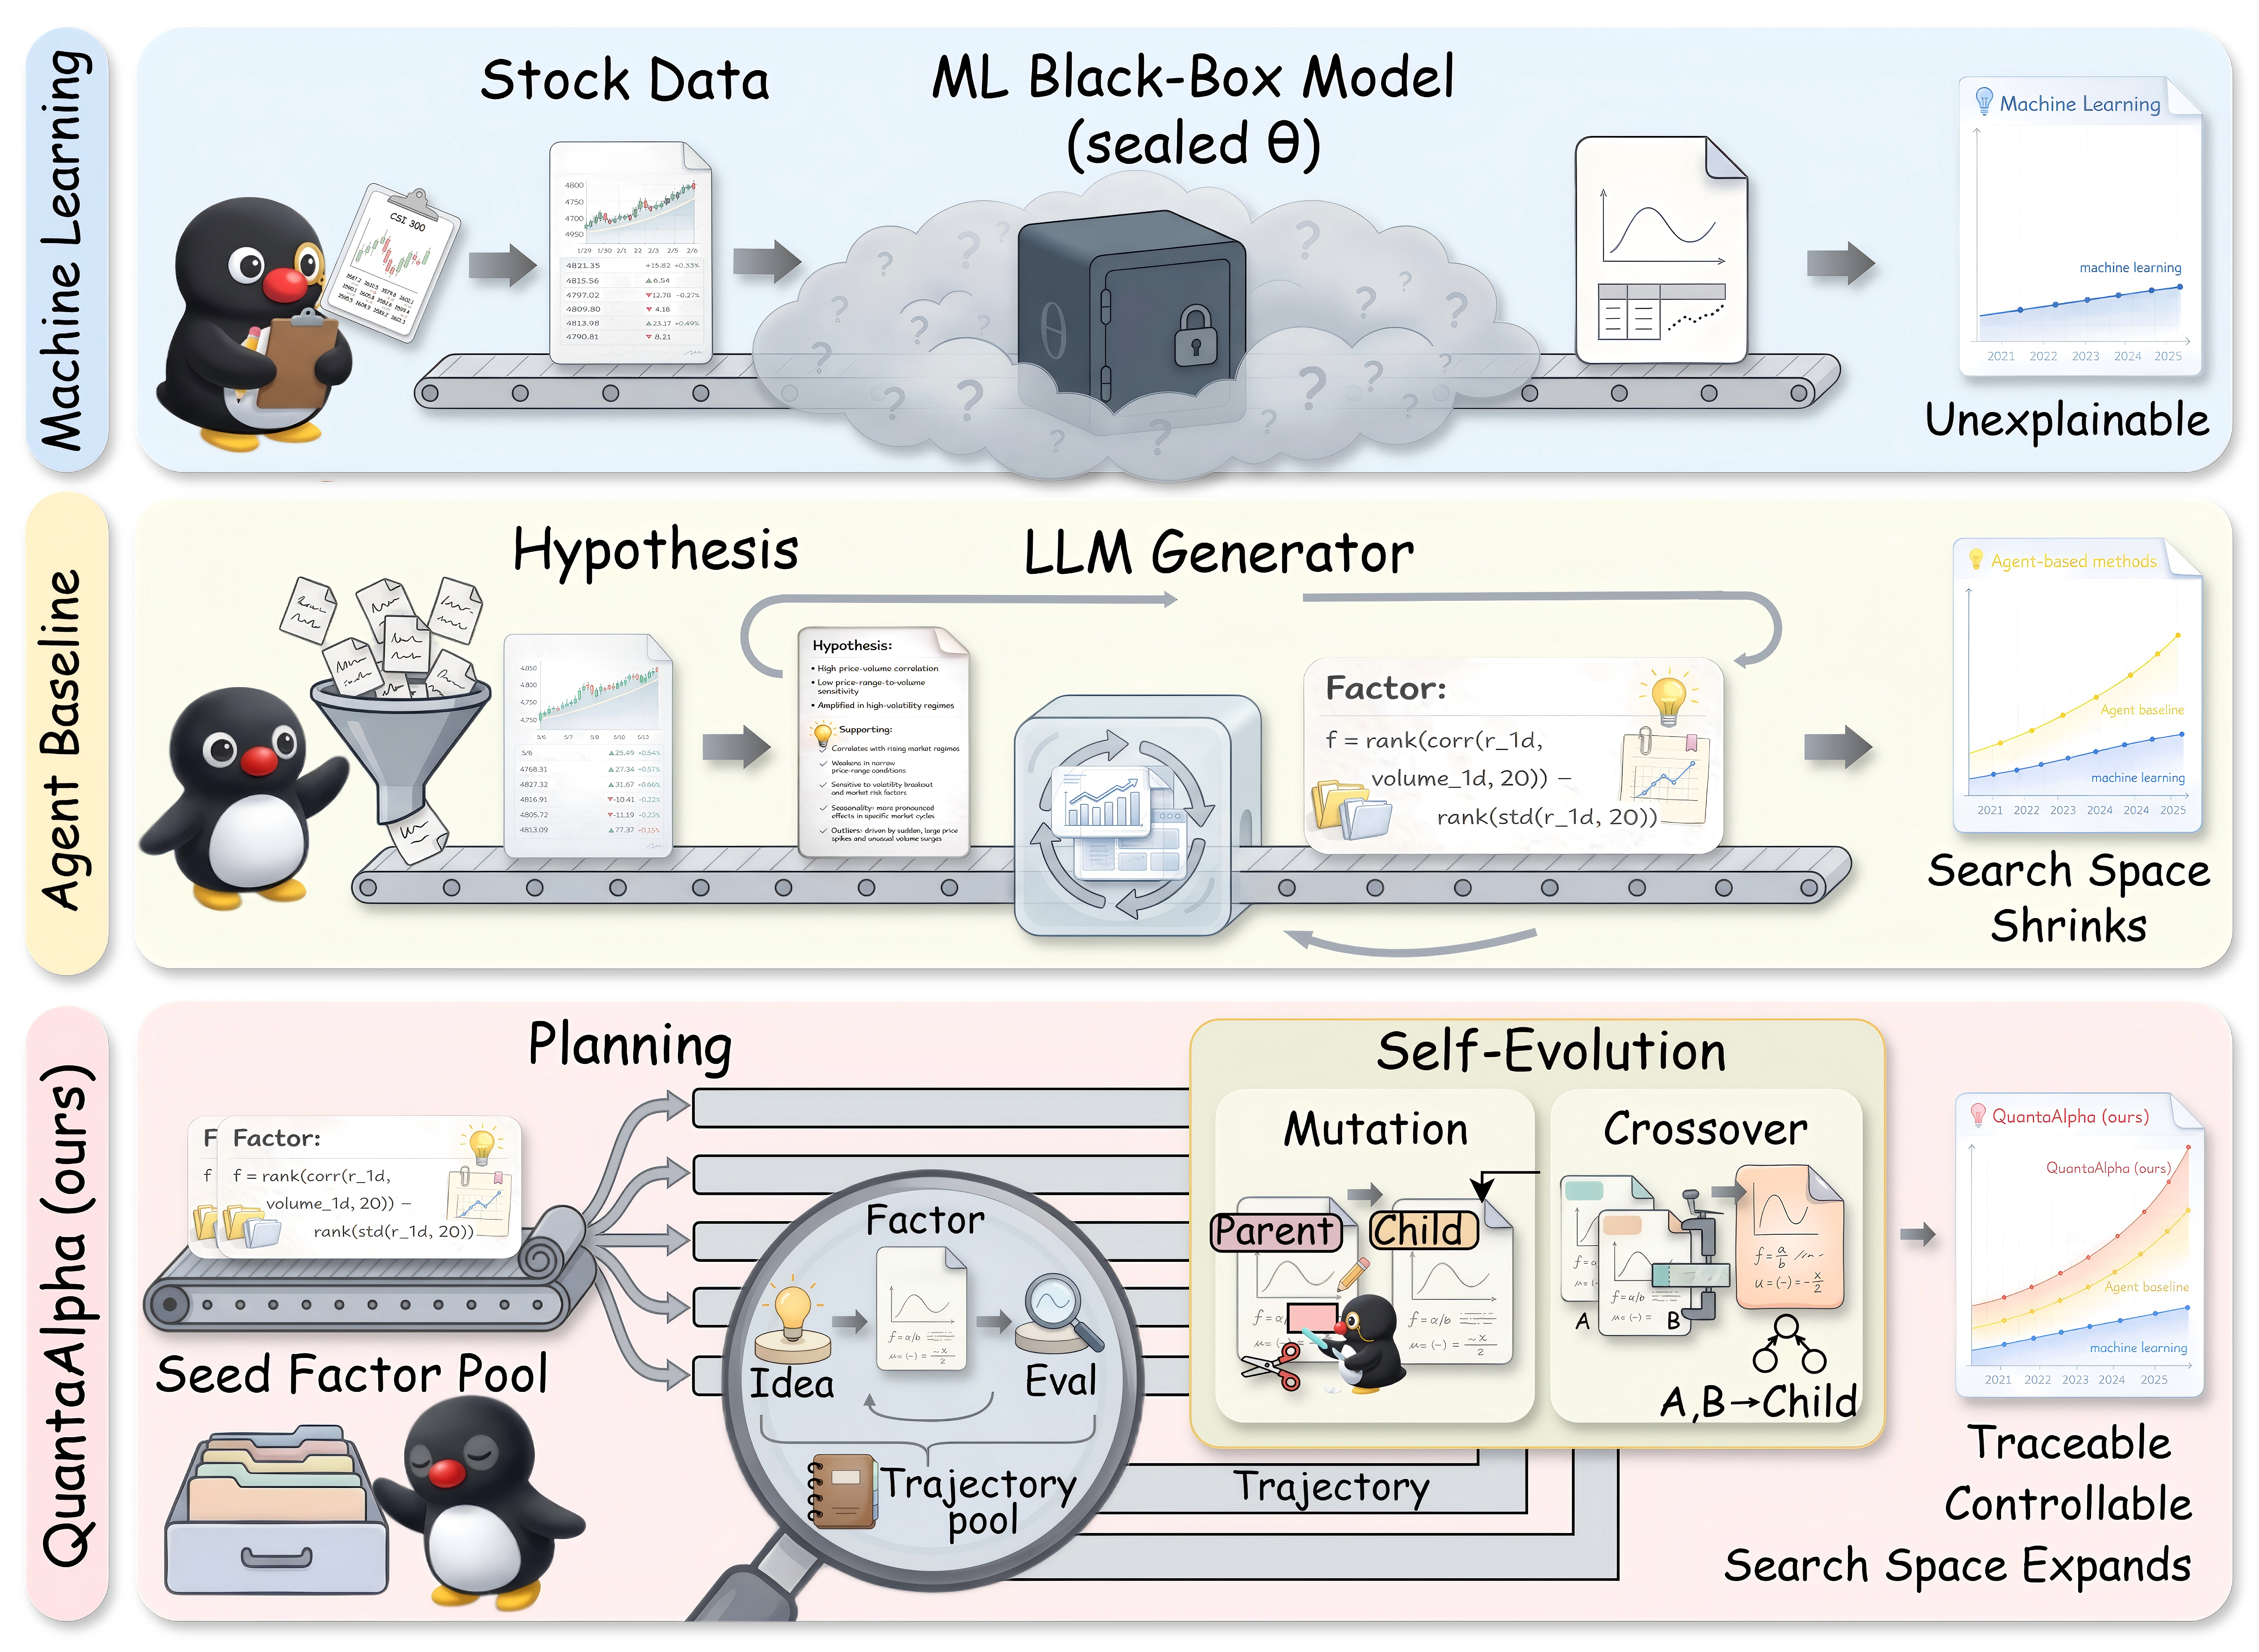
\includegraphics[width=0.8\linewidth]{images/Intro.jpg}
    \caption{Comparison with existing methods: QuantaAlpha improves alpha discovery through trajectory-level self-evolution.}
    \label{fig:placeholder}
\end{figure}
Representative agent frameworks for alpha mining simulate the workflow of human quantitative researchers by iteratively performing hypothesis generation, executable factor construction, and backtesting-based refinement, as illustrated in Figure~\ref{fig:placeholder}. Under this paradigm, AlphaAgent \cite{Tang2025AlphaAgent} imposes explicit regularization during factor generation to curb factor crowding and mitigate alpha decay, while RD-Agent \cite{li2025rdagent} targets full-stack automation with coordinated research and development agents, enabling joint factor–model co-optimization for robust strategy discovery. These frameworks reduce the trial-and-error costs of factor research while preserving interpretability relative to parameter-trained methods, making large-scale exploration practical.

However, under real-market non-stationarity and low signal-to-noise ratios, existing systems still face three limitations. \textit{(i) Fragile controllability:} Iterative refinement is driven by noisy backtest feedback, which can induce semantic drift and steer updates toward spurious correlations, gradually deviating from the intended economic mechanism. \textit{(ii) Limited trustworthiness:} Many methods rely on stochastic re-generation conditioned on transient contexts, without explicitly inheriting validated rationales across iterations. As a result, they lack a traceable lineage and the produced factors are harder to audit and trust. \textit{(iii) Constrained exploration:} Search often over-exploits local neighborhoods around initial seeds, leading to redundancy and factor crowding, while providing limited systematic coverage of the broader hypothesis space and weakening long-horizon discovery. 

To address these challenges, we propose \method, an evolutionary alpha mining framework that improves factor quality through trajectory-level self-evolution. Inspired by \cite{lin2025se}, we view each end-to-end mining run as a mining trajectory and explicitly evolve trajectories rather than relying on unconstrained re-generation from noisy feedback. First, to mitigate local optimization, we introduce a Diversified Planning Initialization that generates multiple complementary research directions, yielding broad initial coverage in the hypothesis space. Second, to support controllable refinement and reliable reuse of validated experience, \method performs self-evolution via trajectory-level mutation and crossover. Mutation performs targeted revision by localizing the failure-causing step via self-reflection and rewriting only the corresponding segment, while keeping the rest of the trajectory intact. Crossover recombines complementary segments from high-reward parents to reuse validated hypothesis structures, construction patterns, and repair behaviors. We further apply generation constraints to enforce semantic consistency and constrain complexity and redundancy, preventing drift and crowding. Together, these mechanisms expand exploration while stabilizing refinement under real-market noise and non-stationarity. Extensive experiments on CSI 300 and cross-market transfer to CSI 500 and S\&P 500 demonstrate consistent improvements in predictive power and strategy performance over strong baselines and prior agentic systems.